\documentclass[journal]{IEEEtran}

\usepackage[T1]{fontenc}
\usepackage[utf8]{inputenc}
\usepackage{amsmath,amssymb,amsfonts}
\usepackage{graphicx}
\usepackage{booktabs}
\usepackage{cite}
\usepackage{url}
\usepackage{hyperref}
\usepackage{xcolor}
\usepackage{multirow}

\hypersetup{
  colorlinks=true,
  linkcolor=blue,
  citecolor=blue,
  urlcolor=blue
}

\begin{document}

\title{All-Japan-Grid: Automated Extraction of Japan's Nationwide Transmission Grid Topology from OpenStreetMap}

\author{
  \IEEEauthorblockN{Hayashi~(given name TBD) and Ryuto~Shigenobu}
  \IEEEauthorblockA{Department of Electrical, Electronic, and Computer Engineering,\\
  University of Fukui, Fukui, Japan}
}

\markboth{IEEE Open Access, 2026}
{Hayashi and Shigenobu: All-Japan-Grid}

\maketitle

\begin{abstract}
Japan's power system lacks publicly available bus-level network models comparable to FERC Form~715 (U.S.) or ENTSO-E datasets (Europe). This paper presents \textit{All-Japan-Grid}, an open-source pipeline that automatically extracts the geographic topology of Japan's transmission grid from OpenStreetMap~(OSM) crowdsourced data. The resulting dataset covers all 10 regional power systems (50/60~Hz dual-frequency), comprising 6,962~substations, 40,077~transmission lines, and 19,138~power plants. The pipeline incorporates a seven-stage data enrichment process that reduces attribute gaps by 87\%, geographic endpoint matching with Haversine distance for topology construction, and synthetic electrical parameter estimation based on voltage-class reference tables. The framework provides conversion to pandapower and MATPOWER formats, 20~AC power flow solvers, and a mixed-integer linear programming~(MILP) unit commitment solver with storage and inter-regional interconnection constraints. A national-scale unit commitment test with 757~generators across 9~interconnections was solved to optimality in under 10~seconds, revealing a 1.4\% congestion cost premium when transmission constraints are enforced. The framework further closes the operations chain from scheduling to frequency control: the unit commitment solution supplies online inertia and regulation headroom to a multi-area load-frequency control (AGC) simulation whose per-class generator dynamics follow the IEEJ AGC30 standard model, and whose inter-area tie stiffness is measured from the extracted network topology rather than assumed. While the synthetic parameters preclude engineering-grade accuracy, the dataset serves as a reproducible baseline for power systems research, algorithm benchmarking, and educational applications in data-scarce environments.
\end{abstract}

\begin{IEEEkeywords}
Power grid topology, OpenStreetMap, open data, transmission network, pandapower, MATPOWER, unit commitment, power flow analysis
\end{IEEEkeywords}

\IEEEpeerreviewmaketitle

%% ========================================
\section{Introduction}
\IEEEPARstart{J}{apan's} electric power system is operated by 10 regional general electricity transmission and distribution operators spanning a dual-frequency infrastructure: 50~Hz in eastern Japan (Hokkaido, Tohoku, Tokyo) and 60~Hz in western Japan (Chubu and westward), interconnected via three frequency conversion stations with a combined capacity of 2,100~MW~\cite{occto2023}.

Unlike the United States, where FERC Form~715 mandates disclosure of network models, and Europe, where ENTSO-E provides transparency platform data~\cite{entsoe}, Japan has no public obligation to release bus-level transmission models. The Electricity and Gas Market Surveillance Commission~(OCCTO) publishes interconnection capacities and supply-demand plans, but detailed electrical parameters---impedances, transformer characteristics, and nodal demand distributions---remain proprietary.

OpenStreetMap~(OSM)~\cite{osm} provides crowdsourced geographic data for power infrastructure, including substation locations, transmission line routes, and power plant facilities. While OSM captures \textit{geographic topology}---where assets are located and how they connect spatially---it does not contain \textit{electrical parameters}. This paper presents an automated pipeline that bridges this gap by: (1)~extracting geographic topology from OSM, (2)~enriching missing attributes through multi-source geocoding, (3)~estimating synthetic electrical parameters, and (4)~providing analysis-ready models in standard formats.

The contributions of this work are:
\begin{enumerate}
  \item A fully automated, reproducible pipeline for extracting Japan's nationwide transmission grid topology from public OSM data.
  \item A seven-stage attribute enrichment process achieving 87\% gap reduction using Overpass API, MLIT P03 facility data, and Nominatim geocoding.
  \item Integration of 20~AC power flow solvers, a MILP-based unit commitment solver with inter-regional transmission constraints, and a multi-area AGC (load-frequency control) simulation layer that consumes the UC solution directly --- closing the operations chain UC $\to$ power flow $\to$ AGC on the same dataset.
  \item A national-scale dataset with 6,962~substations, 40,077~lines, and 19,138~plants, openly available for research and education.
\end{enumerate}

%% ========================================
\section{Related Work}

\subsection{Open Power Grid Datasets}
Several open datasets exist for international benchmarking. The IEEE test cases (14, 30, 118, 300-bus)~\cite{ieee_testcase} provide canonical benchmarks but lack geographic grounding. PyPSA-Eur~\cite{pypsa_eur} constructs a European transmission model from ENTSO-E data. The U.S. Synthetic Grid project~\cite{birchfield2017} generates geographically realistic test networks. For Japan, no comparable open dataset exists at the transmission level.

\subsection{OSM for Power Infrastructure}
Arderne et al.~\cite{arderne2020} demonstrated OSM-based extraction of African power grids for electrification planning. Medjroubi et al.~\cite{medjroubi2017} used OSM for German grid modeling in the SciGRID project. These efforts validate OSM as a viable data source, though data completeness varies significantly by region.

\subsection{Power Flow and Unit Commitment}
pandapower~\cite{pandapower} provides Python-based power system modeling with Newton-Raphson and fast-decoupled solvers. MATPOWER~\cite{matpower} is the standard MATLAB tool for power flow and OPF. Unit commitment formulations using MILP are well-established~\cite{padhy2004}.

%% ========================================
\section{Data Collection Pipeline}

\subsection{Overpass API Extraction}
Three categories of power infrastructure are extracted via the Overpass API~\cite{overpass}: substations (\texttt{power=substation}), transmission lines (\texttt{power=line/cable}), and power plants (\texttt{power=plant}).

Each region is subdivided into an $N \times M$ tile grid to avoid Overpass query timeouts. Inter-query intervals of 3~s comply with API rate limits, with exponential backoff on HTTP~429 responses. Tile-boundary deduplication is performed via OSM~ID matching.

\subsection{Attribute Enrichment}
Raw OSM data contains significant attribute gaps: 49,384 empty names, 41,563 missing operators, and 334 unknown fuel types across 10 regions. A seven-stage enrichment pipeline reduces these gaps by 87\%:

\begin{enumerate}
  \item \textbf{Baseline audit}: Identify and categorize missing attributes.
  \item \textbf{Name promotion}: Nominatim reverse geocoding generates substation names.
  \item \textbf{P03 matching}: Spatial join with MLIT P03 facility dataset provides plant names, operators, fuel types, and capacities.
  \item \textbf{Overpass tag query}: Batch retrieval of OSM tags (500-ID batches).
  \item \textbf{Nominatim geocoding}: Reverse geocoding for fallback names.
  \item \textbf{Line endpoint labeling}: Nearest-substation matching (50~km threshold) generates line names as ``\{from\}--\{to\}.''
  \item \textbf{Fuel normalization}: A 44-entry mapping table standardizes fuel-type variations.
\end{enumerate}

%% ========================================
\section{Topology Construction}

\subsection{Endpoint Matching}
OSM transmission lines lack explicit bus connectivity; only geographic LineString coordinates are provided. For each line endpoint, the nearest substation within Haversine distance $d_\text{max} = 50$~km is assigned:
\begin{equation}
  d = 2R\arctan2\!\left(\sqrt{a},\,\sqrt{1-a}\right)
  \label{eq:haversine}
\end{equation}
where $a = \sin^2(\Delta\phi/2) + \cos\phi_1 \cos\phi_2 \sin^2(\Delta\lambda/2)$ and $R = 6{,}371$~km. Self-loops are rejected.

\subsection{Voltage Cleaning and Transformer Insertion}
Raw voltage tags are snapped to valid Japanese standards: 66, 77, 110, 132, 154, 187, 220, 275, or 500~kV. Lines connecting buses with a voltage ratio $\geq$1.5 are reinterpreted as transformers with parameters from a four-tier lookup table (Table~\ref{tab:trafo}).

\begin{table}[t]
  \centering
  \caption{Transformer parameter defaults by voltage class}
  \label{tab:trafo}
  \begin{tabular}{lrrr}
    \toprule
    HV (kV) & $S_n$ (MVA) & $v_k$ (\%) & $v_{kr}$ (\%) \\
    \midrule
    $\geq$275 & 800 & 14.0 & 0.20 \\
    $\geq$154 & 400 & 12.0 & 0.25 \\
    $\geq$110 & 200 & 10.0 & 0.30 \\
    $<$110    & 100 &  8.0 & 0.40 \\
    \bottomrule
  \end{tabular}
\end{table}

\subsection{Connectivity Recovery}
A component-bridging algorithm iteratively connects orphan components to the main network via KD-tree nearest-bus search, inserting estimated lines or transformers for distances up to 300~km. Post-bridging connectivity reaches 99.7\%.

%% ========================================
\section{Electrical Parameter Estimation}

Electrical parameters are assigned from a voltage-class reference table (Table~\ref{tab:line_params}) derived from OCCTO planning documents and utility design standards.

\begin{table}[t]
  \centering
  \caption{Transmission line parameters by voltage class}
  \label{tab:line_params}
  \begin{tabular}{lrrrc}
    \toprule
    $V$ (kV) & $R$ ($\Omega$/km) & $X$ ($\Omega$/km) & $B$ ($\mu$S/km) & $I_\text{max}$ (kA) \\
    \midrule
    500 & 0.012 & 0.290 & 4.10 & 4.0 \\
    275 & 0.028 & 0.325 & 3.85 & 2.0 \\
    154 & 0.050 & 0.380 & 3.50 & 1.0 \\
    110 & 0.055 & 0.385 & 3.45 & 0.9 \\
     66 & 0.120 & 0.400 & 3.20 & 0.6 \\
    \bottomrule
  \end{tabular}
\end{table}

Line susceptance $B$ (S/km) is converted to capacitance for pandapower using $c_\text{nF/km} = B / (2\pi f) \times 10^9$, where $f$ is the regional frequency.

Per-unit conversion for MATPOWER applies numerical stability floors: $x_\text{pu} \geq 0.005$ (lines), $x_\text{pu} \geq 0.03$ (transformers), and impedance ceilings of 2.0~p.u.

%% ========================================
\section{Analysis Tools}

\subsection{AC Power Flow Solvers}
Twenty solvers are implemented across four categories: (1)~pandapower wrappers (NR, GS, FDPF-BX/XB, backward-forward), (2)~custom Newton-Raphson variants (standard, line-search, Iwamoto, rectangular, current-injection, dishonest, Levenberg-Marquardt), (3)~iterative methods (GS, accelerated GS, Jacobi, SOR), and (4)~decoupled methods (FDPF, decoupled NR, continuation PF). All converge on IEEE 14, 118, and 300-bus benchmarks.

\subsection{Unit Commitment Solver}
A MILP formulation minimizes total operating cost:
\begin{equation}
  \min \sum_{g}\sum_{t} \left[ C_f^g p_{g,t} + C_\text{NL}^g u_{g,t} + C_\text{SU}^g v_{g,t} \right]
  \label{eq:uc_obj}
\end{equation}
subject to demand balance, capacity bounds, startup/shutdown logic, minimum up/down times, ramp rates, reserve margins, maintenance windows, and interconnection capacity constraints. Storage models incorporate SOC dynamics with charging/discharging efficiency. The solver uses HiGHS~\cite{highs} as primary backend.

\subsection{Load-Frequency Control (AGC)}
The AGC layer closes the loop from scheduling to frequency control on the same dataset. Each synchronous island (Hokkaido, East 50~Hz, West 60~Hz, Okinawa) is modeled as a set of control areas (TSO zones) in the deviation domain:
\begin{align}
  M_a \frac{d\Delta f_a}{dt} &= \sum_g \Delta P_{m,g} - \Delta P_{L,a} - D_a \Delta f_a - \Delta P_{\text{tie},a}, \label{eq:lfc_swing}\\
  \Delta P_{\text{tie},a} &= \textstyle\sum_b T_{ab}\,(\Delta\delta_a - \Delta\delta_b),
  \label{eq:lfc_tie}
\end{align}
where the inter-area synchronizing coefficient $T_{ab} = S_\text{base}\sum 1/x$ is \emph{measured} from the in-service extracted corridors crossing each area boundary --- a quantity conventional LFC studies must assume, but which the geographic model supplies directly. The area inertia $M_a$ and the regulation headroom of each responding group are taken from the UC solution (online units and base points at the studied hour), so the three layers share one consistent operating point.

Generator dynamics follow the IEEJ AGC30 standard model~\cite{ieej_agc30} in a simplified per-class second-order form (governor and turbine lags with the AGC30 droop, governor-free width, and LFC ramp-rate constants per plant class; nuclear units run governor-free). Secondary control implements tie-line bias control (TBC; flat-frequency control on single-area islands) with the AGC30 LFC constants ($K_P=1.0$, $K_I=0.003\,\mathrm{s}^{-1}$, 10~MW area-regulation deadband, 5~s cycle) and a continuous-time approximation of the 5-minute EDC layer that redispatches the sustained imbalance. All dynamic parameters are typical published values and are labeled as such in the result ledgers; the simulation is a structural demonstration on the open model, not an operational prediction.

\subsection{Inter-Regional Interconnections}
Nine links model Japan's inter-regional transmission (Table~\ref{tab:ic}), including the Hokkaido--Honshu HVDC (900~MW), Tokyo--Chubu frequency converters (2,100~MW), and six AC interconnections, totaling 24,050~MW.

\begin{table}[t]
  \centering
  \caption{Inter-regional interconnections}
  \label{tab:ic}
  \begin{tabular}{llrc}
    \toprule
    From & To & Capacity (MW) & Type \\
    \midrule
    Hokkaido & Tohoku & 900 & HVDC \\
    Tohoku & Tokyo & 5,550 & AC \\
    Tokyo & Chubu & 2,100 & FC \\
    Chubu & Kansai & 2,530 & AC \\
    Chubu & Hokuriku & 1,900 & AC \\
    Kansai & Chugoku & 4,090 & AC \\
    Kansai & Shikoku & 1,400 & AC \\
    Chugoku & Shikoku & 1,200 & AC \\
    Chugoku & Kyushu & 2,780 & AC \\
    \midrule
    \multicolumn{2}{l}{\textbf{Total}} & \textbf{24,050} & --- \\
    \bottomrule
  \end{tabular}
\end{table}

%% ========================================
\section{Results}

\subsection{Dataset Statistics}
Table~\ref{tab:dataset} summarizes the extracted dataset. Total coverage: 6,962 substations, 40,077 lines, 19,138 plants, with approximately 274~GW total generation capacity.

\begin{table}[t]
  \centering
  \caption{Dataset statistics by region}
  \label{tab:dataset}
  \begin{tabular}{lrrrr}
    \toprule
    Region & Subs. & Lines & Plants & Freq. \\
    \midrule
    Hokkaido  &    471 &  4,136 &    436 & 50 Hz \\
    Tohoku    &    901 &  6,628 &  1,311 & 50 Hz \\
    Tokyo     &  1,726 &  8,295 &  7,207 & 50 Hz \\
    Chubu     &  1,163 &  6,589 &  3,792 & 60 Hz \\
    Hokuriku  &    267 &  2,296 &    432 & 60 Hz \\
    Kansai    &    902 &  3,994 &  1,518 & 60 Hz \\
    Chugoku   &    531 &  3,176 &  1,173 & 60 Hz \\
    Shikoku   &    258 &  1,532 &    688 & 60 Hz \\
    Kyushu    &    684 &  3,314 &  2,581 & 60 Hz \\
    Okinawa   &     59 &    117 &    --- & 60 Hz \\
    \midrule
    \textbf{Total} & \textbf{6,962} & \textbf{40,077} & \textbf{19,138} & --- \\
    \bottomrule
  \end{tabular}
\end{table}

\subsection{National Unit Commitment}
A 757-generator, 10-region, 24-hour UC was solved with and without interconnection constraints (Table~\ref{tab:uc}). All nine interconnections reached 100\% utilization under peak demand.

\begin{table}[t]
  \centering
  \caption{National unit commitment results}
  \label{tab:uc}
  \begin{tabular}{lrr}
    \toprule
    Scenario & Cost (\textyen B) & Time (s) \\
    \midrule
    Copper plate (no limits) & 7.65 & 9.28 \\
    With interconnection limits & 7.76 & 8.72 \\
    \midrule
    Congestion premium & +1.40\% & --- \\
    \bottomrule
  \end{tabular}
\end{table}

\subsection{Operations Chain: UC $\to$ Power Flow $\to$ AGC}
Fig.~\ref{fig:agc} and Table~\ref{tab:agc} close the chain on one consistent operating point per synchronous island: the UC solution at the island peak hour fixes the online fleet (inertia, headroom) and the largest online plant; the extracted network verifies the dispatch (full AC power flow converges on all four synchronous islands --- including the 7,928-bus west island, which becomes AC-solvable after two disclosed interventions: territory re-attribution of extraction-overlap nodes restricted to prefectures with a unique mains frequency, and eight ledgered \emph{provisional} infeed transformers that assert only the electrically necessary existence of an upper-grid path to served metropolitan load pockets missing from OSM --- with the DC snapshot retained as fallback, 100\,\% served on all four islands) and supplies the measured inter-area stiffness ($T_{ab}$ of $2\times10^2$--$1.6\times10^4$~pu/rad; the weakest western corridor, Kansai--Shikoku at 206~pu/rad, correctly identifies the thin Honshi link). Because these measured stiffnesses place inter-area swing modes far above the LFC band, the AGC layer uses a coherent-island reduction with tie-flow deviations recovered algebraically; swing dynamics proper remain the domain of the transient-stability suite.

Two disturbances are simulated per island. A 2\,\%-of-demand load step --- the standard LFC benchmark --- is restored to within $\pm$0.02~Hz in 198--788~s by TBC with AGC30 constants, with the disturbed area absorbing the full correction and neighboring-area commands returning to zero (Fig.~\ref{fig:agc}c). The largest-online-plant trip is an \emph{upper bound} of unit-level $N$-1 (the P03-derived generator granularity is one plant, not one unit) and is run with a typical-value three-step \emph{latching} UFLS (relays shed and stay shed): the two large islands absorb their worst plant loss with nadirs of $-1.4$/$-1.1$~Hz without shedding, while on Hokkaido the loss of the To\-ma\-to-atsuma plant (1,650~MW on a 4.4~GW, 14.3~GW$\cdot$s system) drives $-$2.9~Hz/s RoCoF to a $-$2.5~Hz nadir; only shedding 1,141~MW of load arrests the fall, after which frequency rebounds and recovers slowly --- structurally consistent with the September 2018 Hokkaido blackout sequence.

\begin{figure*}[t]
  \centering
  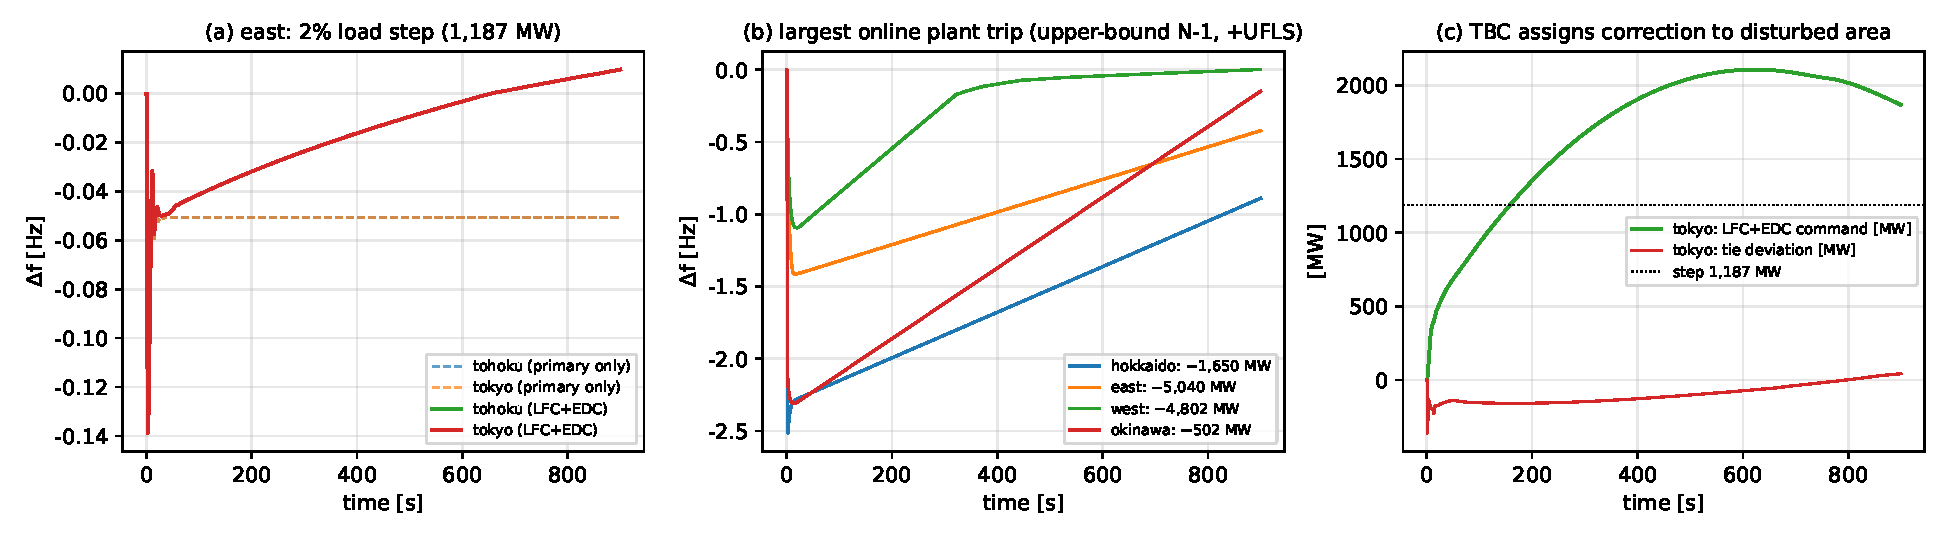
\includegraphics[width=\textwidth]{figs/fig_agc.pdf}
  \caption{UC $\to$ PF $\to$ AGC chain. (a)~2\,\% load step on the east island: primary response settles at the analytic $-\Delta P/\beta$ offset (dashed); LFC+EDC restores frequency. (b)~Largest-online-plant trip per island with typical-value UFLS. (c)~Under TBC the disturbed area's command converges to the lost power while its tie deviation and the neighboring areas' commands return to zero. All generator/control constants follow the IEEJ AGC30 standard model~\cite{ieej_agc30}; parameters are typical published values (structural demonstration, not an operational study).}
  \label{fig:agc}
\end{figure*}

\begin{table}[t]
  \centering
  \caption{AGC chain at island peak hour (UC scenario FY2023)}
  \label{tab:agc}
  \begin{tabular}{lrrrr}
    \toprule
     & Hokkaido & East & West & Okinawa \\
    \midrule
    Peak demand (MW) & 4,434 & 59,353 & 69,938 & 1,682 \\
    Online inertia (GW$\cdot$s) & 14.3 & 245.6 & 332.5 & 6.3 \\
    Largest online plant (MW) & 1,650 & 5,040 & 4,802 & 502 \\
    Trip RoCoF (Hz/s) & $-$2.88 & $-$0.51 & $-$0.43 & $-$2.39 \\
    Trip nadir (Hz)$^{\dagger}$ & $-$2.51 & $-$1.41 & $-$1.09 & $-$2.31 \\
    2\,\% step restore (s) & 240 & 347 & 788 & 198 \\
    \bottomrule
  \end{tabular}

  \vspace{2pt}
  {\footnotesize $^{\dagger}$Plant-granularity trip (upper bound of unit $N$-1), with a three-step latching typical-value UFLS active on all islands (shed load does not restore within the simulation).}
\end{table}

%% ========================================
\section{Limitations}

This dataset is generated from crowdsourced OSM data and has inherent limitations: (1)~line impedances and transformer characteristics are synthetic estimates; (2)~endpoint matching may produce false connections ($\sim$2--3\% error rate); (3)~some operators, fuel types, and capacities remain unknown; (4)~no breaker-level data for contingency analysis; (5)~nodal demand uses voltage-class weights rather than measured profiles; the west-island AC solution relies on provisional infeed links whose routes and ratings are explicitly marked as unverified in the model and result ledgers (to be replaced if actual routes are published), and retains large balancing slack (13\% of demand at peak) with local low-voltage pockets; (6)~all AGC dynamic parameters (inertia constants, droop, governor/turbine lags, UFLS settings) are typical published values --- the frequency-response results are structural demonstrations, and generator granularity is plant-level, so trip scenarios upper-bound unit $N$-1. The dataset is suitable for research and education, but \textbf{not} for operational planning.

%% ========================================
\section{Conclusion}

This paper presented \textit{All-Japan-Grid}, an automated pipeline producing the first openly available geographic representation of Japan's 10-region, dual-frequency transmission grid from OSM data. The dataset (6,962 substations, 40,077 lines, 19,138 plants) with 20 power flow solvers and MILP unit commitment provides a research-ready baseline. A national UC test demonstrated optimality in under 10~s with 1.4\% congestion cost, and the operations chain now extends through power-flow verification to multi-area AGC: the same UC solution supplies inertia and regulation headroom to an IEEJ-AGC30-based load-frequency simulation whose inter-area coupling is measured from the extracted network. Future work includes supplementation with official OCCTO data for engineering-grade accuracy.

The dataset and code are available at \url{https://github.com/lutelute/All-Japan-Grid}.

%% ========================================
\begin{thebibliography}{13}

\bibitem{occto2023}
OCCTO, ``Wide-area system long-term plan,'' 2023.

\bibitem{entsoe}
ENTSO-E, ``Transparency platform,'' \url{https://transparency.entsoe.eu}

\bibitem{osm}
OpenStreetMap contributors, ``OpenStreetMap,'' \url{https://www.openstreetmap.org}

\bibitem{overpass}
Overpass API, \url{https://overpass-api.de}

\bibitem{ieee_testcase}
R.~D.~Christie, ``Power systems test case archive,'' Univ. Washington.

\bibitem{pypsa_eur}
J.~H\"{o}rsch \textit{et al.}, ``PyPSA-Eur: An open optimisation model of the European transmission system,'' \textit{Energy Strategy Rev.}, vol.~22, pp.~207--215, 2018.

\bibitem{birchfield2017}
A.~B.~Birchfield \textit{et al.}, ``Grid structural characteristics as validation criteria for synthetic networks,'' \textit{IEEE Trans. Power Syst.}, vol.~32, no.~4, pp.~3258--3265, 2017.

\bibitem{arderne2020}
C.~Arderne \textit{et al.}, ``Predictive mapping of the global power system using open data,'' \textit{Sci. Data}, vol.~7, no.~19, 2020.

\bibitem{medjroubi2017}
W.~Medjroubi \textit{et al.}, ``Open data in power grid modelling,'' \textit{Energy Rep.}, vol.~3, pp.~14--21, 2017.

\bibitem{pandapower}
L.~Thurner \textit{et al.}, ``pandapower---An open-source Python tool for convenient modeling, analysis, and optimization of electric power systems,'' \textit{IEEE Trans. Power Syst.}, vol.~33, no.~6, pp.~6510--6521, 2018.

\bibitem{matpower}
R.~D.~Zimmerman \textit{et al.}, ``MATPOWER: Steady-state operations, planning, and analysis tools,'' \textit{IEEE Trans. Power Syst.}, vol.~26, no.~1, pp.~12--19, 2011.

\bibitem{padhy2004}
N.~P.~Padhy, ``Unit commitment---A bibliographical survey,'' \textit{IEEE Trans. Power Syst.}, vol.~19, no.~2, pp.~1196--1205, 2004.

\bibitem{ieej_agc30}
IEEJ Technical Committee on Standard Analytical Models for Power Supply-Demand Analysis, ``Standard analytical models for power supply-demand and frequency simulations (AGC30),'' IEEJ Technical Report no.~1386, 2016 (in Japanese).

\bibitem{highs}
Q.~Huangfu and J.~A.~J.~Hall, ``Parallelizing the dual revised simplex method,'' \textit{Math. Prog. Comp.}, vol.~10, pp.~119--142, 2018.

\end{thebibliography}

\end{document}
